%	勾股定理测试

%	latex命令宏格式:用花括号括起来
%		1.\command 
%		2.\command <arg1>...
%		3.\command[<arg_opt>]<arg1>...

%	latex环境格式
%		\begin{环境名称}
% 			内容...
%		\end{环境名称}
%		\begin{环境名称}[可选参数](其他参数)
% 			内容...
%		\end{环境名称}

%	latex数学公式表示方式:
%		1.正文公式(行内公式):$  “  ->中间是公式<-  ”      $
%		2.显示公式:
%					\begin{equation}
%						a + b
%					\end{equation}

%	latex插入图表方式:插图是由praphicx提供的
%		方式一:预先图片,需要在\documentclass后边提供\usepackage{graphicx},可以使用\includegraphicx插图
%		方式二:绘制图片
%		\begin{figure}[ht]	% 通用大图居中法,ht浮动
%			\centering	% 后续居中
%			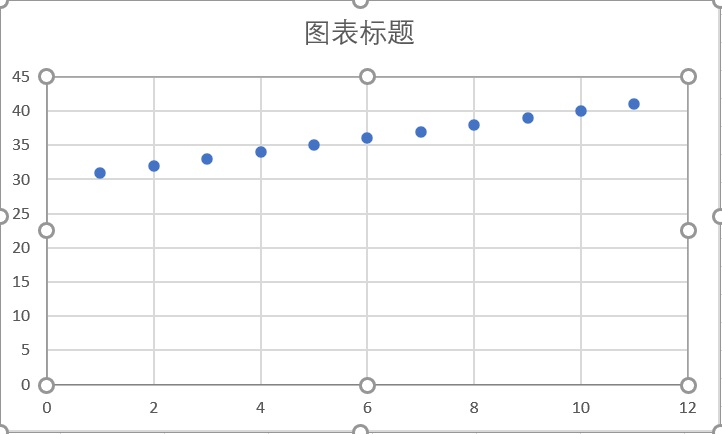
\includegraphics[scale=0.3]{1.jpg}
%			\caption{第一次插图}		% 插入编号标题
%			\label{fig:ope}	% 定义标签,方便引用
%		\end{figure}

\documentclass[UTF8]{ctexart}	% 中文短文 utf-8编码格式
\usepackage{graphicx}	% 插入图片的宏包
\usepackage{subfigure}
\graphicspath{{figs/}}

\usepackage{geometry}	% 设计页面尺寸
\geometry{a4paper,centering,scale = 0.8}

\usepackage[format=hang,font=small,textfont=it]{caption} % 修改图表标题

\newenvironment{myquote}	% 修改散乱格式
	{\begin{quote}\heiti\zihao{-5}}{\end{quote}}
	
\newcommand \degree{^\circ}	% 转化°指令为degree

\usepackage[nottoc]{tocbibind}	% 增加目录项目

\title{\heiti 勾股定理}	% 文章标题 作者 时间
\author{\heiti 张三}
\date{\heiti \today}

\bibliographystyle{plain}	% 声明参考文献格式

% 以上为导言区域
\begin{document}	% 论文正文

\maketitle	% 实际输出论文标题

\begin{abstract}
	围绕国家和陕西省在医药卫生健康领域重大战略需求,以服务国家战略为使命、以解决临床需求为初心、以影像技术发展为指引、以国家重大项目为依托,针对重大疾病早期精准诊疗前沿科学问题,围绕早期病变的精确有效定量,立足信息技术手段,从微观-宏观两个尺度、细胞-动物-人体三个层面研究多尺度定量光学分子成像技术,内容涵盖成像系统、成像理论、定量方法、图像分析、分子探针以及生物基础与转化医学应用。
	\footnote{这都是啥呀}	% 上边的一个脚注
\end{abstract}

\tableofcontents	% 输出目录

\section{方向一}	% 练习引用,改变字体
1.基于拉曼效应的高分辨率动态光谱成像技术
•多尺度多模态拉曼-光学投影成像\emph{技术}	% 改变字体,强调 “技术”二字\\
•快速高分辨率相干拉曼显微成像技术(基于Raman tag的多色/多通道免标记成像)
\begin{myquote}
\centering	% 引用内容,无参数
\zihao{-5} \kaishu	% 修改字号,字体	% 时间这里的 “--”表示宽度
—————————————我是引用内容,(时间6 -- 7年)———————————————
\end{myquote}
•基于拉曼探针的连续波受激拉曼散射显微镜
•基于贝塞尔光束的便携式拉曼光谱成像仪。
\footnote{这都是啥呀}	% 上边的一个脚注

\section{方向二}	% 练习设置定理,插入数学公式
1.基于拉曼效应的高分辨率动态光谱成像技术

\newtheorem{thm1}{定理}	% 使用定理环境,名字是定理,thm1类
\begin{thm1}[bala定理]\label{eq:lalala}
	啦啦啦我是定理一 $a + b$	% 正文公式
	
	\begin{equation}	% 行内公式
		\angle abc = \pi / 2	% \pi \angle
	\end{equation}
	
	\begin{equation}	% 行内公式
	\angle abc = 90^\circ	% 读数
	\end{equation}
	
	\begin{equation}	% 行内公式
	\angle abc = 90\degree	% 读数
	\end{equation}
	
	\begin{equation}	% 行内公式
	a^2 + b^2 = c^{31}		% ^是上标,多个数字是需要加{}
	\end{equation}
	
	\begin{equation}	% 行内公式
	a_2 + b_2 = c_2		% _是上标
	\end{equation}
	
\end{thm1}

•多尺度多模态拉曼-光学投影成像技术
•快速高分辨率相干拉曼显微成像技术
•基于拉曼探针的连续波受激拉曼散射显微镜,式\ref{eq:lalala}
•基于贝塞尔光束的便携式拉曼光谱成像仪。

\section{方向三}	% 练习插入图
1.基于拉曼效应的高分辨率动态光谱成像技术
% 插入图片
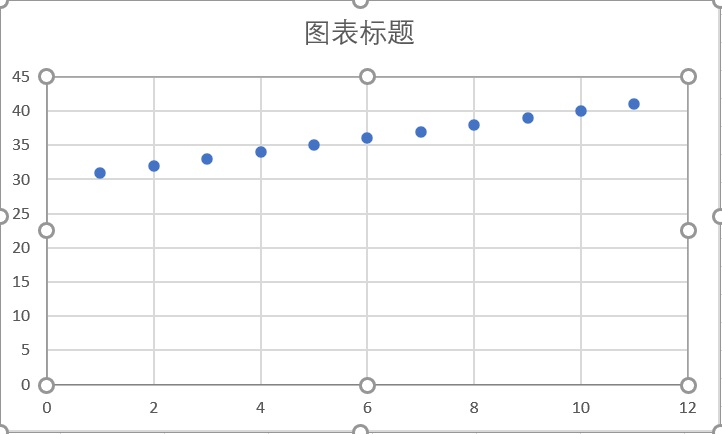
\includegraphics[width=1cm]{1.jpg}	% 小图标插图法

\begin{figure}[ht]	% 通用大图居中法,ht浮动
	\centering	% 后续居中
	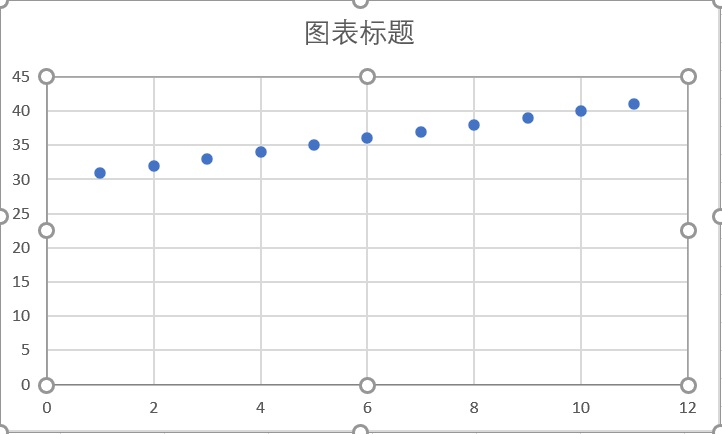
\includegraphics[scale=0.3]{1.jpg}
	\caption{第一次插图}		% 插入编号标题
	\label{fig:ope}	% 定义标签,方便引用
\end{figure}

•多尺度多模态拉曼-光学投影成像技术
•快速高分辨率相干拉曼显微成像技术
•基于拉曼探针的连续波受激拉曼散射显微镜
•基于贝塞尔光束的便携式拉曼光谱成像仪。

\section{方向四}
1.基于拉曼效应的高分辨率动态光谱成像技术
% 插入表格	\\ 隔离行   & 隔离列
\begin{table}[ht]
	\centering
	\begin{tabular}{|rrr|}
		\hline	% 横线
		直角边 $a$ & 直角边 $b$ & 直角边 $c$	\\	
		\hline
		3& 4& 5 \\
		5& 12& 13 \\
		\hline
	\end{tabular}
\end{table}
•多尺度多模态拉曼-光学投影成像技术,图\ref{fig:ope}
•快速高分辨率相干拉曼显微成像技术
•基于拉曼探针的连续波受激拉曼散射显微镜
•基于贝塞尔光束的便携式拉曼光谱成像仪。\cite{KILE}	% 参考文献引用
\bibliography{document}		% 打印参考文献列表
	
\end{document}